\documentclass[pdf,bluish,slideColor,colorBG]{prosper}
\hypersetup{pdfpagemode=FullScreen}
\usepackage{color}
\usepackage{graphicx}
\usepackage{amsfonts}
\usepackage{amsmath}
\def\baselinestretch{0.7}
\parindent 0.3in
\hyphenpenalty=10000
\tolerance=10000
\pagestyle{empty}

\def\Prob{{\rm Prob\;}}
\def\prob{{\rm \;Prob\;}}
\def\Var{{\rm Var}}        % Var
\def\Cov{{\rm Cov}}        % Cov

\DeclareSymbolFont{AMSb}{U}{msb}{m}{n}
\DeclareMathSymbol{\expect}{\mathalpha}{AMSb}{'105}

% bold math (use \bm{...})
\def\bm#1{\mathpalette\bmstyle{#1}}
\def\bmstyle#1#2{\mbox{\boldmath$#1#2$}}

\title{Brownian motion models, multiple characters, and phylogenies}

\author{Joe Felsenstein}

\institution{NIMBioS Evol Quant Gen tutorial}

\subtitle{\small \\ 13 August 2015}


\definecolor{orange}{rgb}{1.0,0.8,0.0}
\definecolor{Dandelion}{rgb}{0.8,0.4,0.3}
\definecolor{golden}{rgb}{1.0,0.75,0.2}
%\definecolor{golden}{rgb}{1.0,0.8,0.3}
\definecolor{purple}{rgb}{0.6,0.2,0.6}
\definecolor{darkblue}{rgb}{0.1,0.1,0.6}
\definecolor{yellow}{rgb}{1.0,1.0,0.0}
\definecolor{brightred}{rgb}{1.0,0.,0.0}
\definecolor{black}{rgb}{0.0,0.0,0.0}
\definecolor{white}{rgb}{1.0,1.0,1.0}
\definecolor{purple}{rgb}{0.8,0.0,0.8}

% sets backgroundcolor for whole document 
%\pagecolor{darkblue}
%\pagecolor{white}
% sets text color
%\color{yellow}
%\color{black}
% to change just a few words
% using \textcolor{color}{text}

\DeclareSymbolFont{AMSb}{U}{msb}{m}{n}
\DeclareMathSymbol{\expect}{\mathalpha}{AMSb}{'105}

\def\Prob{{\rm Prob\;}}
\def\prob{{\rm \;Prob\;}}
\def\Var{{\rm Var}}        % Var
\def\Cov{{\rm Cov}}        % Cov

\begin{document}

% OUTLINE ALL TALKS
% Brownian motion approximation
% Edwards and Cavalli-Sforza
% me, 1968/1973
% Lande, 1976 
% REML trees with Brownian motion
% Pruning
% Inferring the covariances?
% incl. Grafen (and/or PGLS)
% The determinant result (make sure Jacobian included)
% Some kind of simulation with finite number of loci w/mutation
% 
% Source of covariation (VA, selective)
% 
% Ornstein-Uhlenbeck (Marguerite?)
% Chasing a peak
% Go where peak goes
% Smoothing caused by this
% Equilibrium covariances
% Tree covariation
% 
% Morphometrics
% Bookstein
% Alignment
% Rotation and optimization (and approximations)
% Need for special models

% Threshold models
% Sewall Wright( and guinea pig)
% 


\maketitle

{\parindent=0in
\begin{slide}[Replace]{What will approximate change of quantitative characters? }
\bigskip

\begin{itemize}
\item ... when it occurs by genetic drift of pre-existing alleles?
\item ... when it also occurs by mutation to new alleles?
\item ... when variable selection affects the alleles at each locus?
\item ... when selection is on the fitness based on the whole phenotype?
\end{itemize}

\end{slide}

\begin{slide}[Replace]{Approximating genetic drift of two alleles}
\bigskip

Can we compute transition probabilities for genetic models such as the
Wright-Fisher model? 
\begin{itemize}
\item Can we do this analytically? {\bf No.} (although the right eigenvectors and 
the eigenvalues are known) the full set of left eigenvalues has never been derived.
\item We can take such a model for a given (not-too-big) population size $~\mathsf{N}~$ and compute the transition probability matrix, then either power it
up numerically or get its eigenvalues and eigenvectors
\item OK, what about the diffusion approximation.  Aren't they very close
approximations?  Yes, they and Kimura (1955a, 1955b) derived transition 
probabilities for the diffusion process as sums of series in Gegenbaur 
polynomials. {\bf But} they are difficult to work with.
\end{itemize}

\end{slide}

\begin{slide}[Replace]{Edwards and Cavalli-Sforza's approximation}

\centerline{
\begin{tabular}{c c c}
\includegraphics[width=0.5in]{cavedwards3.ps} &
\hspace{0.2in} &
\includegraphics[width=0.8in]{edwards6.ps}\\
Luca Cavalli-Sforza (and Edwards), 1963 & & Anthony Edwards, 1970 
\end{tabular}`
}
\bigskip

The expectation of gene frequency change in one generation (under pure genetic 
drift without mutation) is zero.  The variance is the binomial variance
\[
\mathsf{\expect\left[\left(\Delta p \right)^2\right] \ = \ \frac{p(1-p)}{2N_e}}
\]
\bigskip

That variance is not constant: it varies with $~\mathsf{p}~$ (in a parabola), but maybe we can roughly
approximate it by dealing with the case where all populations have roughly
similar gene frequencies, so the variances are nearly the same.  Maybe.  Roughly.

\end{slide}

\begin{slide}[Replace]{How good is this? }

\centerline{\includegraphics[width=2.9in,angle=-90]{gt5010.ps}}

Starting with $~\mathsf{p\;=\;0.5}$, after 10 generations in a population
of size 50.

\end{slide}

% \begin{slide}[Replace]{How good is this? (we can simulate)}
% \bigskip
% 
% (Break here to run a case in {\tt PopG})
% 
% \end{slide}
% 
% \begin{slide}[Replace]{How good is this? }
% 
%\centerline{\includegraphics[width=2.9in,angle=-90]{gt5020.ps}}
%
%Starting with $~\mathsf{p\;=\;0.5}$, after 20 generations in a population
%of size 50.
%
%\end{slide}
%

\begin{slide}[Replace]{How good is this? }

\centerline{\includegraphics[width=2.9in,angle=-90]{gt5050.ps}}

Starting with $~\mathsf{p\;=\;0.5}$, after 50 generations in a population
of size 50.

\end{slide}

%\begin{slide}[Replace]{How good is this? }
%
%\centerline{\includegraphics[width=2.9in,angle=-90]{gt3010.ps}}
%
%Starting with $~\mathsf{p\;=\;0.3}$, after 10 generations in a population
%of size 50.
%
%\end{slide}
%
%\begin{slide}[Replace]{How good is this? }
%
%\centerline{\includegraphics[width=2.9in,angle=-90]{gt3020.ps}}
%
%Starting with $~\mathsf{p\;=\;0.3}$, after 20 generations in a population
%of size 50.
%
%\end{slide}
%
%\begin{slide}[Replace]{How good is this? }
%
%\centerline{\includegraphics[width=2.9in,angle=-90]{gt3050.ps}}
%
%Starting with $~\mathsf{p\;=\;0.3}$, after 50 generations in a population
%of size 50.
%
%\end{slide}
%

\begin{slide}[Replace]{How good is this? }

\centerline{\includegraphics[width=2.9in,angle=-90]{gt1010.ps}}

Starting with $~\mathsf{p\;=\;0.1}$, after 10 generations in a population
of size 50.

\end{slide}

\begin{slide}[Replace]{How good is this? }

\centerline{\includegraphics[width=2.9in,angle=-90]{gt1020.ps}}

Starting with $~\mathsf{p\;=\;0.1}$, after 20 generations in a population
of size 50.

\end{slide}

%\begin{slide}[Replace]{The arc-sine square-root transform}
%\bigskip
%
%Can't we use the arc-sine square-root transform to homogenize the variance of
%the change in gene frequency?
%\bigskip
%
%Approximately, when $~\mathsf{N}~$ is large.
%\bigskip
%
%It involves following the transformed variable
%\[
%\mathsf{y \ = \ \sin^{-1} \left(\sqrt{p} \right)}
%\]
%
%A ``delta-method'' approximation (basically, the Taylor series) does get
%the standard result for one generation:
%\[
%\mathsf{~\Var(\Delta y) \ \simeq  \frac{1}{8N}}
%\]
%
%\end{slide}
%
%\begin{slide}[Replace]{Trouble in paradise? }
%\bigskip
%
%Taking the Taylor series in $~\mathsf{\Delta y}$, and taking expectations,
%we find that the first term in $\mathsf{~(p-p_0)~}$ is zero, but the second term gives
%\[
%\mathsf{\expect[\Delta y ] \ \simeq \ \expect[\left(p - p_0\right)^2] \frac{2p_0 - 1}{\left(p_0(1-p_0)\right)^{3/2}}}
%\]
%
%and substituting the formulas for variance of gene frequency change this becomes
%\[
%\mathsf{\expect[\Delta y] \ \simeq \ \frac{1}{8N} \frac{2p_0 - 1}{\sqrt{p_0(1-p_0)}}}
%\]
%so there is a directional pressure away from gene frequency $~\mathsf{1/2}$: $~\mathsf{y}~$ is not very well approximated by Brownian Motion.
%\bigskip
%
%So we need the approximation that the gene frequencies are fairly
%similar; this breaks down as they approach 0 or 1.
%
%\end{slide}
%

\begin{slide}[Replace]{What about a quantitative character? }
\bigskip

If a quantitative character is a sum of contributions from a number of loci,
then if the individual locus gene frequencies have their change approximated
by Brownian Motion, the linear combination will also change by Brownian motion.
This works for multiple alleles.
\bigskip

\begin{itemize}
\item if there is any dominance, there will
be some nonlinearity and the approximation will be less good.
\item Epistasis can cause even more trouble.
\end{itemize}

First discussed by me (Felsenstein, 1973).

\end{slide}

\begin{slide}[Replace]{But, if there are mutations making incremental changes .. }
\bigskip

\centerline{\includegraphics[width=3.5in]{mutationscale.idraw}}
\bigskip

... as we saw with the discussion of quantitative characters, if a relatively
constant genetic variance is maintained, and mutations have additive
effects, then
genetic drift will cause the mean to change in a random walk close to Brownian Motion.
\bigskip

{\it However}, if one approaches some limit where most
mutations oppose movement to it, and there are
no mutations allowing you to go past that limit, this approximation
will be poor.

\end{slide}

%\begin{slide}[Replace]{Variable selection as a cause of Brownian Motion }
%\bigskip
%
%I suggested (Felsenstein, 1973) that another cause for Brownian Motion
%would be variable selection, where the selection coefficients change
%through time in a random way (themselves approximating a Brownian Motion).
%\bigskip
%
%Issues with this include:
%\begin{itemize}
%\item The variance of selection coefficients might differ from locus to
%locus
%\item Selection might actually be on the whole character value, rather than
%locus by locus
%\end{itemize}
%
%\end{slide}
%

\begin{slide}[Replace]{Is the Brownian Motion approximation tractable? }
\bigskip

Yes.
\bigskip

You can easily compute transition probabilities from one value to another.
\bigskip

This makes it possible to compute likelihoods on phylogenies, which allows
both likelihood inference and Bayesian inference.
\bigskip

\end{slide}

\begin{slide}[Replace]{Brownian motion along a tree}
\bigskip

Brownian motion for time $~\mathsf{t}~$ has expectation zero and variance
(say) $~\mathsf{\sigma^2}$ per unit time.
\bigskip

So the displacement after time $~\mathsf{t}~$ is normal with expectation
$~\mathsf{0}~$
and variance $~\mathsf{\sigma^2\,t}$.
\bigskip

Displacements in successive periods are independent, and when they are
added up, the overall expectation is still $~\mathsf{0}~$ and the
variance is $~\mathsf{\sigma^2\,(t_1\,+\,t_2\,+\,t_3)}$.


\end{slide}

\begin{slide}[Replace]{Brownian motion along a tree}

\centerline{\includegraphics[height=0.7in]{brownian2.idraw}}

\vspace{-0.15in}
\[
\begin{tabular}{l l c r c}
Where & $\mathsf{\Delta x_1 \: = \: x_1 - x_0}$,& ~~~~ & Note that\hspace{0.2in} &   $\mathsf{x_2 \ = \ x_0 +  \Delta x_1 + \Delta x_2}$\\

& $\mathsf{\Delta x_2 \: = \: x_2 - x_1}$, etc. & &  and\hspace{0.2in}      &   $\mathsf{x_3 \ = \  x_0 + \Delta x_1 + \Delta x_3 }$
\end{tabular}
\]

\vspace{-0.05in}
where each of the displacements $~\mathsf{\Delta x_i}~$ is normally distributed, independently,
with mean $~\mathsf{0}~$ and variance $~\mathsf{v_i}$. 
\medskip

The covariance (noting that $~\mathsf{x_0}~$ is constant and drops out) is
\[
\begin{array}{l c l}
\mathsf{\Cov(x_2, x_3)} & \mathsf{=} & \mathsf{\Cov(\Delta x_1\;+\;\Delta x_2, \ \ \Delta x_1\;+\; \Delta x_3)}\\[3pt]
&   \mathsf{=} &  \mathsf{\Cov(\Delta x_1,\ \Delta x_1) \ + \Cov(\Delta x_1,  \Delta x_2)}\\
&     &   \mathsf{\ + \ \Cov(\Delta x_1, \Delta x_3) \ + \ \Cov(\Delta x_2, \Delta x_3)}
\end{array}
\]

\vspace{-0.10in}
and, since changes in different branches are independent, this is 

\vspace{-0.05in}
\[
\mathsf{\Cov(x_2, x_3) \ =  \Cov(\Delta x_1, \Delta x_1) \ + 0 \ + \ 0 \ + \ 0 \ = \
\Var(\Delta x_1) \ = \ v_1}
\]

\end{slide}

\begin{slide}[Replace]{Brownian motion along a tree}

\centerline{\includegraphics[height=3.0in]{fig23-1.ydraw}}

\end{slide}

\begin{slide}[Replace]{Covariances of species on the tree}
\bigskip

{\ptsize{8}
\[
\hspace*{0in}\hspace{-0.34in}\left[\hspace{-0.1in}
\begin{array}{c c c c c c c c c c c c c}
\multicolumn{3}{c}{\mathsf{v_1+v_8+v_9}} & \mathsf{v_8+v_9} & & \mathsf{v_9} & & \mathsf{0} & & \mathsf{0} & & \mathsf{0} & \mathsf{0} \\
& \mathsf{v_8+v_9} & \multicolumn{3}{c}{\mathsf{v_2+v_8+v_9}} & \mathsf{v_9} & & \mathsf{0} & & \mathsf{0} & & \mathsf{0} & \mathsf{0}\\
& \mathsf{v_9}     & & \mathsf{v_9} & \multicolumn{3}{c}{\mathsf{v_3+v_9}} & \mathsf{0} & & \mathsf{0} & & \mathsf{0} & \mathsf{0} \\
& \mathsf{0}       & & \mathsf{0} & & \mathsf{0} & \multicolumn{3}{c}{\mathsf{v_4+v_{12}}} & \mathsf{v_{12}} & & \mathsf{v_{12}} & \mathsf{v_{12}} \\
& \mathsf{0}       & & \mathsf{0} & & \mathsf{0} & & \mathsf{v_{12}} & \multicolumn{3}{c}{\mathsf{v_5+v_{11}+v_{12}}} & \mathsf{v_{11}+v_{12}} & \mathsf{v_{11}+v_{12}} \\
& \mathsf{0}       & & \mathsf{0} & & \mathsf{0} & & \mathsf{v_{12}} & & \mathsf{v_{11}+v_{12}} & \multicolumn{2}{c}{\mathsf{v_6+v_{10}+v_{11}+v_{12}}} & \mathsf{v_{10}+v_{11}+v_{12}} \\
& \mathsf{0} & & \mathsf{0} & & \mathsf{0} & & \mathsf{v_{12}} & & \mathsf{v_{11}+v_{12}} & \multicolumn{2}{c}{\mathsf{v_{10}+v_{11}+v_{12}}} & \mathsf{v_7+v_{10}+v_{11}+v_{12}} \\
\end{array}\hspace{-0.05in}\right]
\]
}

\end{slide}

\begin{slide}[Replace]{Covariances are of form }
\bigskip

{\ptsize{10}
\[
\left[
\begin{array}{c  c c | c c c c}
\multicolumn{1}{c|}{\mathsf{a}} & \multicolumn{1}{c|}{\mathsf{b}} & \mathsf{c} & \mathsf{0} & \mathsf{0} & \mathsf{0} & \mathsf{0} \\
\cline{1-2}
\multicolumn{1}{c|}{\mathsf{b}} & \multicolumn{1}{c|}{\mathsf{d}} & \mathsf{c} & \mathsf{0} & \mathsf{0} & \mathsf{0} & \mathsf{0} \\
\cline{1-3}
\mathsf{c} & \multicolumn{1}{c|}{\mathsf{c}} & \mathsf{e} & \mathsf{0} & \mathsf{0} & \mathsf{0} & \mathsf{0} \\
\hline
\mathsf{0} & \mathsf{0} & \mathsf{0} & \multicolumn{1}{c|}{\mathsf{f}} & \mathsf{g} & \mathsf{g} & \mathsf{g} \\
\cline{4-7}
\mathsf{0} & \mathsf{0} & \mathsf{0} & \multicolumn{1}{c|}{\mathsf{g}} & \multicolumn{1}{c|}{\mathsf{h}} & \mathsf{i} & \mathsf{i} \\
\cline{5-7}
\mathsf{0} & \mathsf{0} & \mathsf{0} & \multicolumn{1}{c|}{\mathsf{g}} & \multicolumn{1}{c|}{\mathsf{i}} & \multicolumn{1}{c|}{\mathsf{j}} & \mathsf{k} \\
\cline{6-7}
\mathsf{0} & \mathsf{0} & \mathsf{0} & \multicolumn{1}{c|}{\mathsf{g}} & \multicolumn{1}{c|}{\mathsf{i}} & \multicolumn{1}{c|}{\mathsf{k}} & \mathsf{l} \\
\end{array}
\right]
\]
}

\end{slide}

\begin{slide}[Replace]{An outcome of Brownian motion on a 5-species tree}

\centerline{\includegraphics[height=3.0in]{fig23-2a.ydraw}}

\end{slide}

\begin{slide}[Replace]{An outcome of Brownian motion on a 5-species tree}

\centerline{\includegraphics[height=3.0in]{fig23-2b.ydraw}}

\end{slide}

\begin{slide}[Replace]{An outcome of Brownian motion on a 5-species tree}

\centerline{\includegraphics[height=3.0in]{fig23-2c.ydraw}}

\end{slide}

\begin{slide}[Replace]{An outcome of Brownian motion on a 5-species tree}

\centerline{\includegraphics[height=3.0in]{fig23-2.ydraw}}

\end{slide}

%\begin{slide}[Replace]{ML, REML, biases etc. }
%
%(See Chapter 23 of my book for details)
%
%Careful algebra on the two-species case with $\mathsf{p}$ independently
%evolving Brownian traits shows:
%
%\begin{itemize}
%\item If you try to estimate two branch lengths plus the starting coordinate
%at each character, the whole problem blows up (likelihoods go to $\mathsf{\infty}$).
%\item If you constrain the two branch lengths to be equal (a morphological
%clock) their values are underestimated twofold.
%\item You can cure all this by using only the differences $\mathsf{x_1 - x_2}$ and discarding the mean $\mathsf{(x_1+x_2)/2}$.
%\item The expectation of the difference is zero, so you no longer have an extra
%parameter for each coordinate that undergoes Brownian Motion.
%\item This means you no longer have a number of parameters which rises with the
%number of characters.
%\item It is not ML but is REML.
%\end{itemize}
%
%\end{slide}
%
%\begin{slide}[Replace]{ ``Pruning'' a tree in the Brownian motion case}
%
%In 1967 for my thesis, I wondered whether taking the difference
%of the values in sister species would simplify things.  For the example tree:
%\[
%\mathsf{\Var(x_1 - x_2) \ = \ (v_1 + v_8 + v_9) \ + \ (v_2 + v_8 + v_9) \ - \ 2 (v_8 + v_9) \ = \  v_1 + v_2}
%\]
%\noindent
%(so just the branch lengths between nodes 1 and 2).
%\medskip
%
%Can we replace $~\mathsf{x_1}~$ and $~\mathsf{x_2}~$ with their difference and
%some sort of mean?  
%Is there a weighted average of $\mathsf{x_1}$ and $\mathsf{x_2}$ that is independent of this?  Yes!
%
%{\ptsize{8}
%\[
%\renewcommand{\arraystretch}{1.25}
%\begin{array}{c c l}
%\mathsf{\Cov[\:a x_1 + (1-a) x_2, \ \ x_1 - x_2]} & \mathsf{=} &  \mathsf{a\,\Var(x_1) - (1-a) \Var(x_2) + (1-2a) \Cov(x_1, x_2)}\\[3pt]
%& \mathsf{=} & \mathsf{a (v_1 + v_8 + v_9) \ - \ (1-a) (v_2 + v_8 + v_9)}\\
%&  &  \mathsf{\ + \ (1-2a) (v_8 + v_9)}\\[3pt]
%& \mathsf{=} & \mathsf{a\,v_1  \ - \ (1-a)\,v_2} \\
%\end{array}
%\]
%}
%
%\noindent
%which is zero if ~~$\mathsf{a = v_2 / (v_1 + v_2)}$.  In effect, $\mathsf{x_1}$ is weighted by the inverse of its variance, $\mathsf{1/v_1}$.
%
%
%\end{slide}
%

\begin{slide}[Replace]{ ``Pruning'' a tree in the Brownian motion case}
\bigskip

One can take two neighboring tips, and consider their difference $\ \mathsf{x_1 -
x_2\ }$ as well as a weighted average $\ \mathsf{a x_1 + (1-a) x_2}$.  Using
  weights $\mathsf{a\, :\, 1-a \ = \  1/v_1\, :\, 1 /v_2}$, the weighted average is
independent of the difference, and the difference is also independent of the
rest of the tree.
\bigskip

In fact, this weighted average behaves like a tip:  Its covariances with
the other species are the same as those of $\mathsf{x_1}$ and $\mathsf{x_2}$.
It acts just as if the tree were pruned, cutting off species 1 and 2, leaving
a single species whose variance is a bit bigger.
\bigskip

\[
\mathsf{\Var[a x_1 + (1-a) x_2] \ = \  v_8 + v_9 + \frac{v_1 v_2}{v_1 + v_2}}
\]

so in effect, a small extra amount of branch length is added.

\end{slide}

\begin{slide}[Replace]{ ``Pruning'' a tree in the Brownian motion case}

\centerline{\includegraphics[height=2.2in]{fig23-3.ydraw}}

\medskip
(True in the sense that the REML likelihoods -- which are a bit different than the usual likelihoods -- add up).

\end{slide}

\overlays{5}{
\begin{slide}[Replace] {Can decompose the tree into $~\mathsf{n-1}~$  two-species trees}
\bigskip

\begin{itemstep}
\item As we decompose the tree of $~\mathsf{n}~$ species into $~\mathsf{n-1}~$ two-species trees, we do so simultaneously at all characters.
\item We can then use simple formulas to compute the log-likelihoods of the two-species tree (taking all $~\mathsf{p}~$ characters into account.
\item The REML log-likelihood is the sum of these log-likelihoods.
\item The tree is unrooted, in that where its root is placed does not affect its
log-likelihood.
\item This would also make it easy to optimize branch lengths one at a time to find the (RE)ML estimates of those lengths.  But mostly we get those from molecular data.
\end{itemstep}

\end{slide}

\begin{slide}[Replace]{Covarying character change along a lineage}
\bigskip

What is the distribution of changes in multiple characters (say $\mathsf{p}$
of them) along a lineage?   Simply the appropriate multiple of the
infinitesimal rate of change per unit branch length.
\bigskip

If a set of characters $~\mathsf{\bf x}~$, changes under covarying Brownian 
motion, in time $~\mathsf{t}~$ (or a pseudo-time branch-length $~\mathsf{t}~$ 
) the change will be distributed as

\[
\mathsf{\bf {\Delta x} \ \sim \  {\cal N} (\bf 0, {\bf V}t)},
\]

(where $~\mathsf{\bf V}~$ is the covariance matrix of the infinitesimal change 
of the Brownian Motion).

\end{slide}

\begin{slide}[Replace]{Joint distribution for multiple species, characters}
\bigskip

\centerline{\includegraphics[width=3in]{multibrownian.idraw}}
\bigskip

Consider change of two characters, each assessed in a different species.  Say
character $~\mathsf{x}~$ and character $~\mathsf{y}$, the first measured
in species 2, the second in species 3.   The result will give us the pattern
for any two characters measured in any two species.
\bigskip

\end{slide}


%\begin{slide}[Replace]{Seeing that covariances are zero in different branches ... }
%\bigskip
%
%\[
%\mathsf{\Cov[ \Delta x_1 + \Delta x_2, \ \ \Delta y_1 + \Delta y_3]}
%\]
%
%Given that changes in different branches are independent (whether changes of
%the same character or of different characters), the only nonzero covariance
%is between $~\mathsf{\Delta x_1}~$ and $~\mathsf{\Delta y_1}.$
%
%\[
%\mathsf{\Cov[ \Delta x_1 + \Delta x_2, \ \ \Delta y_1 + \Delta y_3]}
%\]
%
%\[
%\mathsf{ \ = \ \Cov[ \Delta x_1, \ \: \Delta y_1]}
%\]
%
%So the covariance of different characters in different species is the
%product of the shared evolution to their common ancestor by the
%(infinitesimal) covariance of the character change per unit branch length.
%
%\end{slide}
%
%\begin{slide}[Replace]{Joint distribution for many species, many characters}
%\bigskip
%
%The upshot is that if $~\mathsf{x_{ik}}~$ is character $~\mathsf{k}~$ in species$~\mathsf{i}$, and $~\mathsf{x_{j\ell}}~$ is character
%$~\mathsf{\ell}~$ in species $~\mathsf{j}$, the covariance between them is
%\[
%\mathsf{Cov [x_{ik}, x_{j\ell}] \ = \ t_{ij}\;v_{k\ell}}
%\]
%where $~\mathsf{t_{ij}}~$ is the time (branch length) to the latest common ancestor of
%species $~\mathsf{i}~$ and species $~\mathsf{j}$. $\mathsf{\bf V}~$ is the covariance matrix of evolutionary
%change for the characters.
%
%\end{slide}
%
%\begin{slide}[Replace]{A stacked vector with a partitioned covariance matrix}
%\bigskip
%
%We have $~\mathsf{n}~$ species and $~\mathsf{p}~$ characters measured in
%each.  Taking the vector of the $~\mathsf{p}~$ characters for species 1, the
%vector for species 2, and so on and stacking one on top of the other with
%the species in order, we get a column vector (shown here transposed).
%\[
%\mathsf{{\bf x} ^T \ = \ \left(~\mathsf{x_{11}, x_{12}, \dots, x_{1p}\:
%\raisebox{0pt}{|}
%\:  x_{21}, x_{22}, \dots, x_{2p}\: \raisebox{0pt}{|} \: \dots \:
%\raisebox{0pt}{|} \: x_{n1}, x_{n2}, \dots, x_{np}}~\right)},
%\]
%\bigskip
%
%The matrix of covariances of these will be partitioned into $~\mathsf{n}~$
%groups of rows and $~\mathsf{n}~$ groups of columns.
%\bigskip
%
%For each box in the partitioned matrix, we will get a multiple of the
%infinitesimal covariance of characters, the multiple being the branch
%length up to the shared common ancestor of those two species.
%\bigskip
%
%\end{slide}
%
%\begin{slide}[Replace]{The Kronecker product, mostly a bookkeeping device}
%\bigskip
%
%This is the Kronecker product of $~\mathsf{\bf T}~$ and $~\mathsf{\bf V}$, which is simply the partitioned matrix
%\bigskip
%
%\[
%\mathsf{{\bf T} \otimes {\bf V} \ = \ \left[
%\begin{array}{c c c c}
%t_{11}{\bf V} & t_{12}{\bf V} & \dots & t_{1p}{\bf V}\\
%t_{21}{\bf V} & t_{22}{\bf V} & \dots & t_{2p}{\bf V}\\
%\vdots & \vdots & \ddots & \vdots \\
%t_{n1}{\bf V} & t_{n2}{\bf V} & \dots & t_{np}{\bf V}\\
%\end{array}
%\right]
%}
%\]
%
%\noindent
%so that this is an $~\mathsf{np \times np}~$ matrix.
%\bigskip
%
%\end{slide}
%
%\begin{slide}[Replace]{The algebra}
%
%If $\bf{T}$ is the covariances of $~\mathsf{n}~$ tips on the tree, and $\bf{V}$ is the (unknown) covariances of the Brownian motion of the $~\mathsf{p}~$ characters, the log-likelihood of
%a set of characters (stacked as a vector) $\bf{x}$ is
%\[
%\mathsf{\ln L \ = \ - (np/2) \ln (2\pi) - (1/2) \ln |{\bf T}\otimes{\bf V}| -
%(1/2) ({\bf x-\bm{\mu}})^t ({\bf T}\otimes{\bf V})^{-1} ({\bf x-\bm{\mu}})}
%\]
%If ${\bf C}$ is an $~\mathsf{(n-1) \times n}~$ set of contrasts, each
%orthogonal to the grand mean, we have seen that we can choose them so that
%each contrast has mean 0 and variance 1.  Then ${\bf CTC}^t$ is an
%$~\mathsf{n-1}$-dimensional identity matrix.
%\medskip
%
%Taking the density of the transformed data $\mathsf{~{\bf y} = {\bf C} {\bf
%x}~}$ (and not forgetting the term for the
%Jacobian of the transformation), this has expectation vector $\mathsf{\bf 0}$ so that the density
%is
%\vspace{-0.20in}
%
%\[
%\hspace*{0in}\hspace{-0.2in}\mathsf{\ln L \ = \ K - (1/2) \ln |{\bf I}_{n-1}\otimes{\bf V}| - (1/2) {\bf
%y}^t ({\bf I}_{(n-1)}\otimes{\bf V})^{-1} {\bf y} \ - \ \frac{1}{2}
%\sum_{i=1}^{n-1} \ln \left(v_1^{(i)}+v_2^{(i)}\right)}
%\]
%\vspace{-0.20in}
%
%(where $~\mathsf{K}~$ collects the constant stuff and the
%$\mathsf{v_1^{(i)}+v_2^{(i)}}$ is the variance of the $i$th contrast computed
%from $\mathsf{~{\bf T}}$, not from $\mathsf~{\bf V}$).
%
%\end{slide}
%
%% SIMPLIFY THE ABOVE

%\begin{slide}[Replace]{ ... simplifying ... }
%
%This can also be expressed as
%\vspace{-0.10in}
%\[
%\mathsf{\ln L \ = \ K - \frac{(n-1)}{2} \ln |{\bf V}| - (1/2) {\rm tr} \left({\bf S}
%{\bf V}^{-1}) \right) - \frac{1}{2} \sum_{i=1}^{n-1} \ln
%\left(v_1^{(i)}+v_2^{(i)}\right)}
%\]
%where
%\vspace{-0.05in}
%\[
%\mathsf{{\bf S} \ = \ \sum\limits_i {\bf y}^{(i)} \left({\bf y}^{(i)}\right)^t}
%\]
%is the $~\mathsf{p \times p}~$ sum of squares matrix of characters across contrasts. 
%
%Inferring the Brownian motion phylogenetic covariances by maximum likelihood
%we find that
%\[
%\mathsf{\widehat{\bf V} \ = \ {\bf S} / (n-1)}
%\]
%which leads to
%\[
%\mathsf{\ln L \ = \ K' \ - \ \frac{(n-1)}{2} \ln |\widehat{\bf V}|}
%\]
%\noindent
%where $\mathsf{~K'~}$ includes the $\mathsf{~\ln\left(v_1^{(i)}+v_2^{(i)}\right)~}$penalty terms, which don't change if the tree stays the same.
%


\begin{slide}[Replace]{What causes change in quantitative characters? }
\bigskip

For neutral mutation and genetic drift, can show that for a quantitative
character with additive genetic variance $~\mathsf{V_A}~$ and population size $\mathsf{~N~}$
the genetic (additive) value of the population mean is:
\bigskip

\[
\mathsf{\Var (\Delta \bar{g}) \ = \ V_A / N}
\]
\bigskip

If mutation and drift are at equilibrium:
\[
\mathsf{\expect\left[V_A^{(t+1)}\right] \ = \ V_A^{(t)} \left(1 - \frac{1}{2N}\right) + V_M}
\]
\bigskip

\end{slide}

\begin{slide}[Replace]{In neutral traits additive genetic variance rules}
\bigskip

so that
\[
\mathsf{\expect\left[V_A\right] \ = \ 2N V_M}
\]

whereby
\[
\mathsf{\Var[\Delta {\bar g}] \ = \ \left(2N V_M \right) / N  \ = \  2 V_M}
\]

an analog of Kimura's result for neutral mutation.
\bigskip

Thus to transform characters to independent Brownian motions of equal
evolutionary variance, we could use the additive genetic variance $\mathsf{V_A}$.

\end{slide}

\begin{slide}[Replace]{With multiple characters ... }
\bigskip

There is a precise analogue of this for multiple characters:

\[
\mathsf{\expect\left[{\bf A}^{(t+1)}\right] \ = \ {\bf A}^{(t)} \left(1 -
\frac{1}{2N}\right) + {\bf M}}
\]
\noindent
where $\mathsf{~{\bf A}~}$ is the additive genetic covariances, and
$\mathsf{~{\bf M}~}$ is the covariance matrix of pleiotropic effects of
mutation.

\[
\mathsf{\expect\left[{\bf A}\right] \ = \ 2N\, {\bf M}}
\]

\noindent
and

\[
\mathsf{\Var[{\bf \Delta {\bar g}}] \ = \ \left(2N {\bf M} \right) / N  \ = \
2 {\bf M}}
\]
\bigskip

\noindent
so as long as mutations cause expected change zero (i.e. they are not near some
biological limit), the effect of genetic drift is that the mean phenotype
wanders according to the mutational covariances.  The constant additive genetic variance assumption was used by Russ Lande.

\end{slide}

\begin{slide}[Replace]{Let's see ... }
\bigskip

(Pause to run simulation of mutation and genetic drift in two characters).

\end{slide}

\begin{slide}[Replace]{With selection ... life is harder \textcolor{purple}{(REVIEW)} }

There is the ``Breeder's Equation'' of Wright and Fisher (1920's)
\[
\mathsf{\Delta z\ =\ h^2 S}
\]
\vspace{-0.10in}

\centerline{\includegraphics[width=1.0in]{Lande2011.ps}}
\medskip

and Russ Lande's (1976) recasting of that in terms of slopes of mean fitness
surfaces:
\vspace{-0.2in}

\[
\mathsf{S \ =\ V_P \; \frac{d \log\left({\bar w} \right)}{ d\bar{x}  }}
\]
\vspace{-0.2in}

\[
\mathsf{\Delta z\  =\  (V_A/V_P)\; V_P\; \frac{d \log\left({\bar w} \right)}{ d\bar{x} }
= \ V_A\;\frac{d \log\left({\bar w} \right)}{d\bar{x}  }}
\]

\noindent
Note -- it's heritability times the slope of log of {\it mean} fitness with
respect to {\it mean} phenotype.  There is an exact multivariate analog of
this equation.

\end{slide}

\begin{slide}[Replace]{Selection towards an optimum \textcolor{purple}{(REVIEW)} }
\bigskip

\centerline{\includegraphics[width=1.5in]{fig24-1.ydraw}}

If fitness as a function of phenotype is:
\[
\mathsf{w(x)\  = \ \exp\left[-\frac{(x-p)^2}{2 V_s } \right]}
\]
\vspace{-0.1in}

Then after some completing of squares and integrating,
the change of mean phenotype ``chases'' the optimum:
\[
\mathsf{m' - m\  =\  \frac{V_A}{V_s + V_P}\; (p - m)}
\]
\vspace{-0.1in}

\noindent
(There is an exact matrix analog of this for multiple characters).

\end{slide}

\overlays{2}{
\begin{slide}[Replace] {Sources of evolutionary correlation among characters}
\bigskip

Variation (and covariation) in change of characters occurs for two reasons:

\begin{itemstep}
\item {\bf Genetic covariances}. (the same loci affect two or more traits)
\item {\bf Selective covariances} (Tedin, 1926; Stebbins 1950). The same
environmental conditions select changes in two or more traits -- even
though they may have no genetic covariance.
\end{itemstep}

\end{slide}
}

\begin{slide}[Replace]{A simple example of selective covariance}
\bigskip

\noindent
\centerline{\includegraphics[width=4.7in]{selectcov.ydraw}}

\end{slide}

\begin{slide}[Replace]{Chasing a peak, simulated with two characters}
\bigskip

\centerline{\includegraphics[width=2.5in]{fig4.100.idraw}}

Genetic covariances assumed negative, but the wanderings of the adaptive peaks 
assumed positively correlated.  In the first 100 generations the genetic covariances are most influential.

\end{slide}
\begin{slide}[Replace]{Chasing a peak, simulated with two characters}
\bigskip

\centerline{\includegraphics[width=2.5in]{fig4.1000.idraw}}

Genetic covariances assumed negative, but the wanderings of the adaptive peaks 
assumed positively correlated.
After a while (every 10th generation up to generation 1000), the wanderings of the peaks start to be
influential.

\end{slide}

\begin{slide}[Replace]{Chasing a peak, simulated with two characters}
\bigskip

\centerline{\includegraphics[width=2.5in]{fig4.10000.idraw}}

Genetic covariances assumed negative, but the wanderings of the adaptive peaks 
assumed positively correlated.
In the long run (every 100th generation up to generation 10,000) the means go mostly where the peaks go.

\end{slide}

\begin{slide}[Replace]{A case that has received too little attention}
\bigskip

\begin{itemize}
\item Suppose characters $\mathsf{~x~}$ and $\mathsf{~y~}$ are genetically correlated.
\item and $\mathsf{~y~}$ is under optimum selection, but $\mathsf{~x~}$ is the one we observe.
\item What will we see?  In effect, the sum (actually, a weighted average) of
an Ornstein-Uhlenbeck process and Brownian Motion.
\item So Brownian motion restricted in the short run but not in the long run.
\item It will look almost like Ornstein-Uhlenbeck Process with an optimum which wanders by Brownian Motion.
\end{itemize}

Most models so far do not allow for characters that are observed to covary with those that aren't observed.

\end{slide}

\begin{slide}[Replace]{A little algebra showing the effect of selective covariance}
\bigskip

If we start from the familiar ``Breeder's Equation'' of quantitative genetics:
\[
\mathsf{\Delta z \ = \ h^2 \:S}
\]
it has long been known to have a multivariate version:
\[
\mathsf{\bm{\Delta z} \ = \ {\bf G} {\bf P}^{-1} {\bf S}}
\]

Multiplying $\bm{\Delta z}$ by its transpose:
\[
\mathsf{\bm{\Delta z} \bm{\Delta z}^T \ = \ {\bf G} {\bf P}^{-1} {\bf S} {\bf
S}^T {\bf P}^{-1} {\bf G}}
\]
and taking expectations (treating $\mathsf{\bf G}$ and $\mathsf{\bf P}$ as
constants) we get for the mean squares:
\[
\mathsf{\expect[\bm{\Delta z} \bm{\Delta z}^T] \ = \ {\bf G} {\bf P}^{-1} \expect[{\bf S} {\bf S}^T] \bf P^{-1} {\bf G}}
\]

\noindent
(Felsenstein, 1988)

\end{slide}

\begin{slide}[Replace]{A research program? }
\bigskip

What we could imagine doing is:

\begin{itemize}
\item We might hope to infer additive genetic covariances by doing quantitive
genetics breeding experiments to infer them from covariances among relatives,
perhaps even in multiple species.
\item Infer the covariances of the changes along the phylogeny.
\item From them, back-calculate the selective covariances.
\item The genetic covariances may also be inferrable from differences between
nearby tips on the tree if we do not have breeding experiments.
\item There is little or no hope of inferring ``selective correlations''
more directly without a complete understanding of the functional ecology.
\end{itemize}

\end{slide}


%\begin{slide}[Replace]{A tree with punctuated equilibrium}
%\bigskip
%
%\centerline{\includegraphics[height=2.8in]{fig24-2.ydraw}}
%
%\end{slide}
%
%\begin{slide}[Replace]{The punctuated tree when we sample 10 species}
%\bigskip
%
%\centerline{\includegraphics[height=3in]{fig24-3.ydraw}}
%
%\end{slide}
%


\begin{slide}[Replace]{References for genetic drift}

Feller, W. 1951. Diffusion processes in genetics. pp. 227-246 in
{\it Proceedings of the 2nd Berkeley Symposium on Mathematical Statistics and 
Probability}, ed. J. Neyman. University of California Press, Berkeley and Los 
Angeles. \textcolor{purple}{\bf [Feller's partial solution of the pure drift
process for the Wright-Fisher model (and his famous proof that the process
converges to the diffusion process)]}
\medskip

Kimura, M. 1955a. Solution of a process of random genetic drift with a 
continuous model. {\it Proceedings of the National Academy of Sciences}
{\bf 41:} 144-150.
\textcolor{purple}{\bf [Exact solution in Gegenbaur polynomials for two-allele
pure genetic drift in a diffusion process approximation]}
\medskip

Kimura, M. 1955b. Random drift in a multi-allelic locus. {\it Evolution} {\bf
9:} 419-435. \textcolor{purple}{\bf [The same, for three alleles]}
\medskip


\end{slide}

\begin{slide}[Replace]{References for the Brownian Motion approximation}

Edwards, A.W. F. and L. L. Cavalli-Sforza.  1964. Reconstruction of
evolutionary
trees. pp. 67--76 in {\it Phenetic and Phylogenetic Classifcation}, ed. V. H.
Heywood and J. McNeill. Systematics Association Publ. No. 6, London.`
\textcolor{purple}{\bf [The first paper on numerical approaches to phylogeny
reconstruction; uses parsimony and proposes likelihood for gene frequency
trees]}
\medskip

Edwards, A.W. F. 1970. Estimation of the branch points of a branching diffusion
process. {\it Journal of the Royal Statistical Society B} {\bf 32:} 155--174.
\textcolor{purple}{\bf [More detailed consideration of the statistical
properties of a maximum likelihood approach to gene frequency phylogenies]}
\medskip

Felsenstein, J. 1973. Maximum likelihood estimation of evolutionary trees from
continuous characters. {\it American Journal of Human Genetics} {\bf 25:}
471--492. \textcolor{purple}{\bf [REML approach to gene frequency phylogenies,
including the contrasts algorithm for rapid computation of likelihood]}
\medskip

Nielsen, R., J. L. Mountain, J. P. Huelsenbeck, and M. Slatkin.  1998.
Maximum-likelihood estimation of population divergence times and population
phylogeny in models without mutation. {\it Evolution} {\bf 52:} 669-677.
\textcolor{purple}{\bf [Little-noticed but much more exact method that would
require MCMC machinery]}
\medskip

\end{slide}

\begin{slide}[Replace]{References on likelihood of Brownian Motion trees}

Thompson, E. A. 1975. {\it Human Evolutionary Trees}. Cambridge University 
Press, Cambridge \textcolor{purple}{\bf [Thesis monograph on how to infer ML 
phylogenies from gene frequencies, published because it won a Smith's Prize 
at Cambridge University]}
\medskip

Felsenstein, J. 1981. Maximum likelihood estimation of evolutionary trees from
continuous characters. {\it Evolution} {\bf 25:} 471--492.
\textcolor{purple}{\bf [Reworks the 1973 paper with more care and
some additional algorithmics, including discussion of effect of character
covariation]}
\medskip

Felsenstein, J. 1985. Phylogenies from gene frequencies: A statistical problem.
{\it Systematic Zoology} {\bf 34:} 300--311. \textcolor{purple}{\bf [Shows how
gene frequency changes depart from being approximated by Brownian Motion]}
\medskip

Felsenstein, J.  2004.  {\it Inferring Phylogenies.}  Sinauer Associates,
Sunderland, Massachusetts. \textcolor{purple}{\bf [See particularly
chapter 23]}
\medskip

\end{slide}

\begin{slide}[Replace]{References for multivariate Brownian motion}

Felsenstein, J. 1988. Phylogenies and quantitative characters. {\it Annual
Review of Ecology and Systematics} {\bf 19:} 445-471. \textcolor{purple}{\bf [Review with mention of
usefulness of threshold model]}
\medskip

Felsenstein, J. 2002. Quantitative characters, phylogenies, and
morphometrics.pp. 27-44 in {\it Morphology, Shape, and Phylogenetics}, ed.
N. MacLeod. Systematics Association Special Volume Series 64. Taylor
and Francis, London.  \textcolor{purple}{\bf[Review repeating 1988 material and going into some
more detail on the question of threshold models.]}
\medskip

Felsenstein, J. 2004. {\it Inferring Phylogenies}. Sinauer Associates,
Sunderland, Massachusetts.  \textcolor{purple}{\bf[Mentions this model and also sample size
issues in contrasts method]}.
\medskip

Lande, R. 1976. Natural selection and random genetic drift in phenotypic
evolution. {\it Evolution} {\bf 30:} 314-334. \textcolor{purple}{\bf [Lande's classic paper on drift versus
optimum selection]}
\medskip

Lande, R. 1979. The quantitative genetic analysis of multivariate
evolution, applied to brain-body size allometry. {\it Evolution} {\bf 33:} 402-416.
\medskip

% Bookstein, F. L. 1997. {\it Morphometric Tools for Landmark Data}. Cambridge
% University Press, Cambridge.  \textcolor{purple}{\bf[A bit dated now]}
% \medskip
% 
% Dryden, I. L. and K. V. Mardia. 1998. {\it Statistical Shape Analysis}. John Wiley
% \& Sons, Chichester, U.K.  \textcolor{purple}{\bf[Formal derivations for shape methods in case of
% independent measurement error in each landmark]}

\end{slide}

\begin{slide}[Replace]{References}

Lande, R. 1980. The genetic covariance between characters maintained
by pleiotropic mutations. {\it Genetics} {\bf 94:} 203-215.
\medskip

Lynch, M. and W. G. Hill. 1986. Phenotypic evolution by neutral mutation.
{\it Evolution} {\bf 40:} 915-935.
\medskip

Stebbins, G. L. 1950. {\it Variation and Evolution in Plants}. Columbia University
Press, New York. \textcolor{purple}{\bf [Describes selective covariance and cites Tedin (1925) for
it]}
\medskip

Tedin, 0. 1925. Vererbung, Variation, und Systematik der Gattung
{\it Camelina}. {\it Hereditas} {\bf 6:} 275-386.
\medskip

Armbruster, W. S. 1996. Causes of covariation of phenotypic traits among
populations. {\it Journal of Evolutionary Biology} {\bf 9:} 261-276. \textcolor{purple}{\bf [Good exposition of
selective covariance]}

\end{slide}
}
}

\end{document}

